\documentclass[12pt]{article}
\usepackage[utf8]{inputenc}
\usepackage{amsmath}
\usepackage{mathtools}
\usepackage{amsfonts}
\usepackage{lastpage}
\usepackage{tikz}
\usepackage{pdfpages}
\usepackage{gauss}
\usepackage{fancyvrb}
\usepackage{fancyhdr}
\usepackage{graphicx}
\pagestyle{fancy}
\fancyfoot[C]{\footnotesize Page \thepage\ of 10}
\DeclareGraphicsExtensions{.pdf,.png,.jpg}
\title{MatIntroNat}
\author{Nikolaj Dybdahl Rathcke}
\chead{Nikolaj Dybdahl Rathcke (rfq695)}

\begin{document}
\section*{MatIntroNat - Opgave 1}

\subsection*{Opgave 2.1 (3.4.12 TLO)}
Find de komplekse løsninger til ligningen $z^2-2iz-(1+i)=0$. Skriv svaret på formen $a+bi$. Uden brug af elektroniske hjælpemidler.\\
\\
Vi ser, at $a=1, b=-2i$ og $c=-(1+i)$, derved får vi løsningerne:\\
$$z=\frac{-b\pm\sqrt{b^2-4ac}}{2a}$$
$$z=\frac{-(-2i)\pm\sqrt{(-2i)^2-4*1*-(i+1)}}{2*1}$$
$$z=\frac{2i\pm\sqrt{-4+4i+4}}{2}$$
$$z=\frac{2i\pm\sqrt{4i}}{2}$$
Vi bliver derfor nødt til at udregne $\sqrt{4i}$. Da $4i$ har modulus 4 og argument $\pi/2$ har tallet en kvadratrod $w_0$ med modulus $\sqrt{4}=2$ og argument $(\pi/2)/2=\pi/4$. Herved ligger tallet i det øvre halvplan er $\sqrt{4i}=2e^{i\pi/4}=\sqrt{2}+i\sqrt{2}$. Derfor har vi, at:
$$z=\frac{2i\pm(\sqrt{2}+i\sqrt{2})}{2}$$
Som giver løsningerne:
$$z_1=\frac{\sqrt{2}}{2}+i(\frac{\sqrt{2}}{2}+1)\:og\:z_2=-\frac{\sqrt{2}}{2}+i(-\frac{\sqrt{2}}{2}+1)$$
På bilag 1 kan du se hvor $z_1$ samt $z_2$ ligger i det komplekse plan.

\subsection*{Opgave 2.2}
Betrag funktionen
$$f(x)=\frac{2x^2-x-1}{x^2+3x+2},\:\:x\in[0,\infty[$$
\subsubsection*{a}
Plot funktionen med Maple.\\
\\
Herunder ses funktionen plotter i Maple:\\
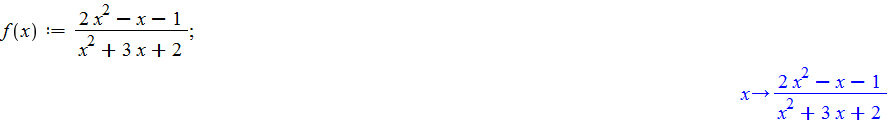
\includegraphics[scale=0.6]{Pic1}\\
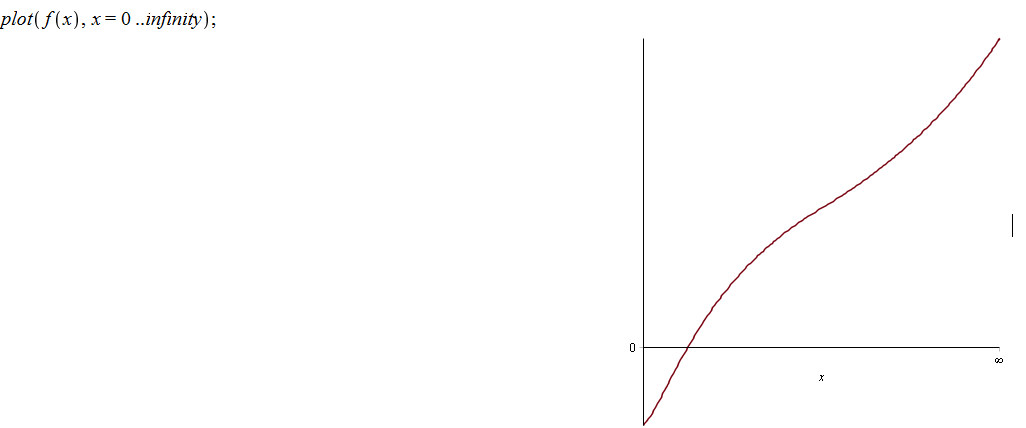
\includegraphics[scale=0.6]{Pic2}

\subsubsection*{b}
Udregn $f'(x)$ og vis at den er positiv for alle $x\in [0,\infty[$.\\
\\
Vi finder først den differentierede og sætter den derefter lig 0 for at finde skæringerne med x-aksen:\\
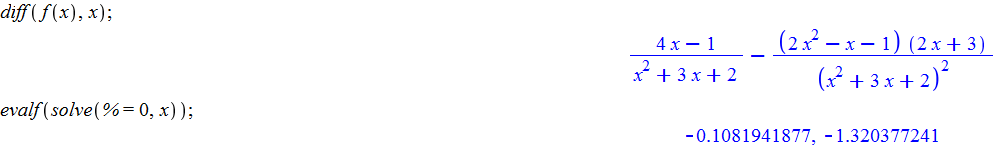
\includegraphics[scale=0.6]{Pic3}\\
Da vi ønsker at kigge på intervallet $x\in[0,\infty[$ og begge skæringer er negative må alle værdier i dette interval nødvendigvis være alle positive eller alle negative. Vi kan derfor blot beregne en værdi af den afledte funktion for at teste dette:\\
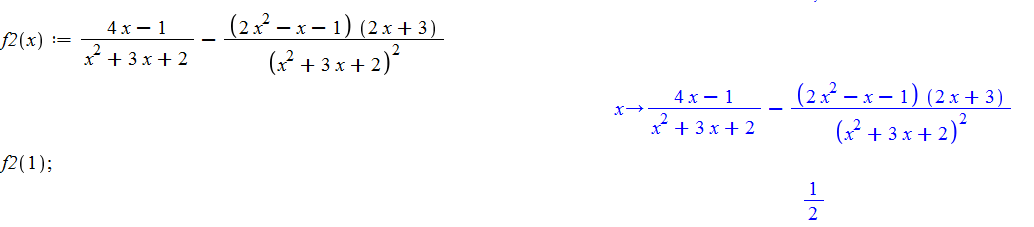
\includegraphics[scale=0.6]{Pic4}\\
Og dermed må den afledte være positiv for $x\in[0,\infty[$

\subsubsection*{c}
Bestem $lim_{n\rightarrow \infty} f(n)$ uden Maple.\\
\\
Vi kigger på funktionen:
$$f(n)=\frac{2n^2-n-1}{n^2+3n+2}$$
Vi ønsker at dividere med $n^2$ i tæller og nævner og får:
$$f(n)=\frac{2n^2/n^2-n/n^2-1/n^2}{n^2/n^2+3n/n^2+2/n^2}=\frac{2-n/n^2-1/n^2}{1+3n/n^2+2/n^2}$$
Nu lader vi $n\rightarrow \infty$ og vi ser leddene i tælleren og nævneren som inkluderer $n$ går mod 0. Derved får vi, at:
$$lim_{n\rightarrow \infty} f(n)=\frac{2}{1}=2$$
Funktionen tilnærmer sig altså 2 når $n$ går mod uendelige.

\subsubsection*{d}
Bestem værdimængden for $f$.\\
\\
Vi har i forrige opgave (c), fundet den øvre grænse for værdimængden til at være 2. Da funktionen er i intervallet $x\in[0,\infty[$ og vi har i opgave (b) vist at den afledte funktion altid er positiv, hvilket vil sige at den er monotont voksende. Vi kan derfor blot beregne $f(0)$ for at finde den nedre grænse:
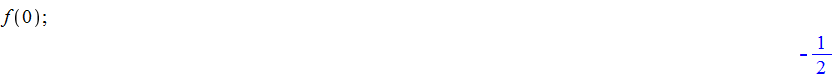
\includegraphics[scale=0.6]{Pic5}\\
Og derfor må værdimængden være $Vm_f=[-\frac{1}{2},2[$.

\subsubsection*{e}
Lad $\epsilon=0.1$. Bestem en værdi af $N$ som kan anvendes i TL definition 4.3.1, når denne definition benyttes på grænseovergangen i (c). Gentag for $\epsilon=0.01$.\\
\\
Vi ønsker at finde et $n\in \mathbb{N}$ således $|a_n-a|<\epsilon$. Vi kender allerede nogle af værdierne og vi skal derfor opfylde:
$$|f(n)-2|<0.1$$
Denne ulighed bruges Maple til at løse:\\
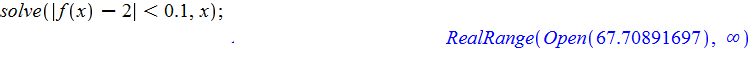
\includegraphics[scale=0.6]{Pic6}\\
Her har jeg fjernet de negative intervaller Maple gav mig da de ikke ligger i definitionsmængden. Vi kan nu blot sætte $n=68$, da det er et naturligt tal og kontrollere svaret:\\
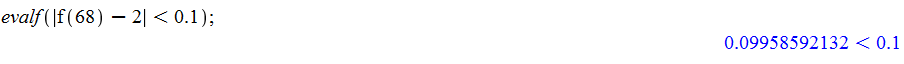
\includegraphics[scale=0.6]{Pic7}\\
Hvilket jo er sandt, og $n=68$ for $\epsilon=0.1$ er derved gyldigt.\\
Vi skal nu prøve det med $\epsilon=0.01$ og til dette har vi samme fremgangsmåde med at finde et $n\in \mathbb{N}$ som opfylder $|f(n)-2|<0.01$:\\
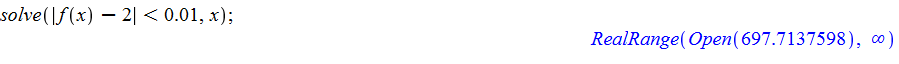
\includegraphics[scale=0.6]{Pic8}\\
Igen er de negative intervallet fjernet da disse ikke ligger i definitionsmængden. Vi kan derfor se at et $n$ større end 697 vil opfylde uligheden. Lad derfor $n=698$ og så kan vi kontrollere svaret:\\
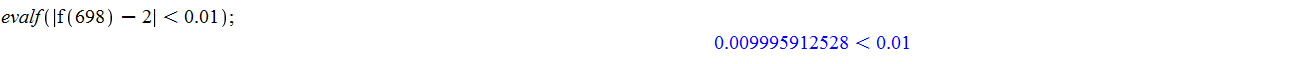
\includegraphics[scale=0.6]{Pic9}\\
Hvilket også er sandt og $n=698$ for $\epsilon=0.01$ er gyldigt.

\subsection*{Opgave 2.3(iv)}
I denne opgave betragter vi hvor hurtigt kaniner kan formere sig under idealiserede forhold. Vi antager at vi starter med et par af nyfødte kaniner,
en han- og en hunkanin. Forestil dig at kaniner kan formere sig når de er
1 måned gamle og en hunkanin har en drægtighedsperiode på 1 måned, så
ved udgangen af den 2. måned kan hun-kaninen føde et nyt kaninpar (men
det nye kuld kommer først til umiddelbart efter 2.måned, således at der i 2.
måned stadig kun er 1 kaninpar.) Vi antager at vores kaniner ikke dør og der
ved hver fødsel kommer et kaninpar bestående af en han- og en hunkanin.
Lad $n \in \mathbb{N}$ betegne måned nummer $n$, med $n = 1$ som den første måned.
Lad $F_n$ betegne antallet af kaninpar i måneden $n$. Hvis kaninerne får lov til
at formere sig frit vil det samlede antal kaninpar være summen af par de to
foregående måneder
$$F_{n+2}=F_n+F_{n+1}$$

\subsubsection*{a}
Giv en intuitiv forklaring på denne rekursionsformel. Hvad er begyndelsesbetingelserne $F_1,F_2$ i vores tilfælde. Bestem hvor mange kaninpar der således vil være efter 1 år.\\
\\
Til en måned $n$ bliver der født lige så mange kaninpar som der var for $n-2$ måneder siden, da alle disse må have født et kaninpar til måneden $n$. Desuden er der også kaninparrene fra $n-1$ måned. Derfor er antallet af kaninpar til en måned $n$ lig summen af de 2 foregående måneder. Altså er $n-2$ antallet af nye kaninpar der bliver født og $n-1$ er antallet af kaninpar der også var der måneden før. De udvikler sig efter fibonacci sekvensen.\\
\\
Begyndelsesværdierne $F_1,F_2$ må være kun vores originale kaninpar, da de første er i stand til at føde i den tredje måned. Altså er $F_1=1$ og $F_2=1$.\\
\\
I maple er rekursionsformlen skrevet ind med begyndelsesværdierne:\\
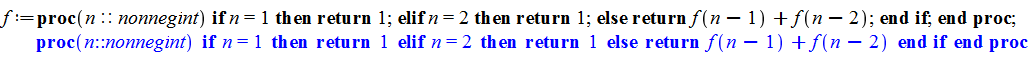
\includegraphics[scale=0.6]{Pic10}\\
Derfra kan vi beregne antallet af kaninpar efter et år. Der er brugt måned 13, da dette tæller som starten af måned 13 og vi begyndte på starten af måned 1:\\
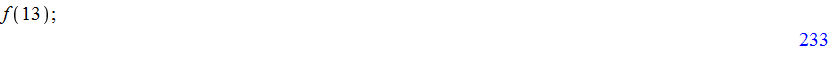
\includegraphics[scale=0.6]{Pic11}\\
Der vil altså være 233 kaninpar efter et år.

\subsubsection*{b}
Vis at elementerne i følgen \{$F_n$\} opfylder for ethvert $n\in \mathbb{N}$
$$F_n\leq F_{n+1}\leq 2F_n$$\\
\\
Vi starter med at vise at den er sand for $n=1$. Der får vi ud fra vores givne begyndelsesværdier:\\
$$F_1\leq F_2\leq 2F_1$$
$$1\leq 1\leq 2$$
Hvilket er sandt. Så antager vi det gælder for alle $n<k$. \\
\\
\textbf{Del 1:} Bevis, at $F(k-1)\leq F(k)$\\
Vi kan opskrive:
$$F(k-2)+F(k-3)\leq F(k-1)+F(k-2)$$
$$F(k-3)\leq F(k-1)$$
Og vi kan derfor konkludere at det må være sandt for $F(k-1)\leq F(k)$.\\
\\
\textbf{Del 2:} Bevis, at $F(n+1)\leq 2*F(n)$\\
Vi kan opskrive:
$$F(k)=F(k-1)+F(k-2)$$
Vi bruger vores antagelse til at sætte en øvre grænse for $F(k-1)$ og $F(k-2)$:
$$F(k-1)\leq 2*F(k-2)$$
$$F(k-2)\leq 2*F(k-3)$$
Hvor der så må gælde, at
$$F(k)\leq 2*F(k-2)+2*F(k-3)$$
$$F(k)\leq 2(F(k-2)+F(k-3))$$
Hvor der kan laves en omskrivning, så
$$F(k)\leq 2*F(k-1)$$
Og derved er det bevist ved induktion, $$F_{n+1}\leq 2F_n$$. En sammenfatning af de 2 delbeviser må vise at,
$$F_n\leq F_{n+1}\leq 2F_n$$
for ethvert $n\in \mathbb{N}$.\\
\\
Vi definerer vækstraten for vores kaninbestand ved:
$$a_n=\frac{F_{n+1}}{F_n}$$
Udregn vækstraten for $n=1,2,..,12$ og plot de beregnede $a_n$ i Maple.\\
\\
Nedenfor er værdierne for $n=1,2,..,12$ angivet og værdierne er plottet ind ved brug af Maple:\\
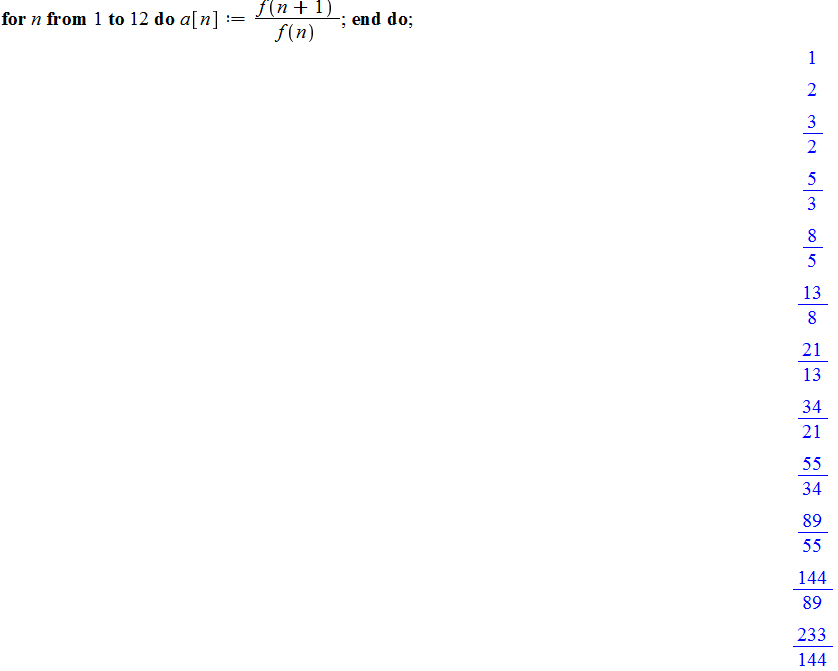
\includegraphics[scale=0.6]{Pic12}\\
\newpage
Plottet i Maple:\\
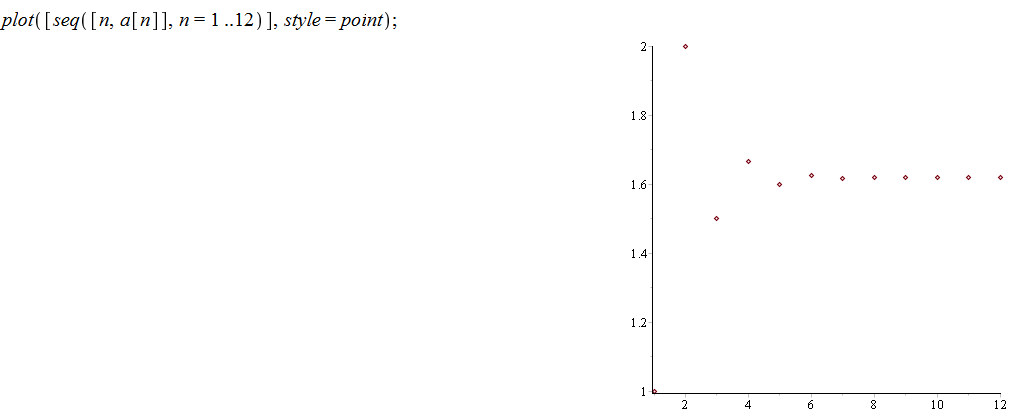
\includegraphics[scale=0.6]{Pic13}
Som viser hvor voksende kaninbestanden er i en måned $n$.

\subsubsection*{c}
Anfør ud fra dit plot i (b) et træk ved den første del af følgen \{$a_n$\}, der taler for at følgen er konvergent. Vi tillader os nu at antage at dette kan uddybes til et bevis for at følgen ER konvergent. Bestem grænseværdien, $a$, af $a_n$ for $n\rightarrow\infty$ uden brug af Maple.\\
\\
Ud fra plottet og de første 12 punkter ses at værdierne nærmer sig en værdi omkring $1.6$. Jo større $n$ bliver, desto tættere ligger punkterne hvilket er et tegn på at den konvergerer mod en bestemt værdi.\\
\\
Denne værdi, grænseværdien, ønsker vi nu at beregne. Fra hintet i opgaven er vi blevet informeret om rekursionsrelationen $a_{n+1}=1+\frac{1}{a_n}$. Ved at kigge på de første værdier:\\
$$a_1=1+\frac{1}{a_0}=1+\frac{1}{0}=1$$
$$a_2=1+\frac{1}{a_1}=1+\frac{1}{1}=2$$
$$a_3=1+\frac{1}{a_2}=1+\frac{1}{2}=\frac{3}{2}$$
$$a_4=1+\frac{1}{a_3}=1+\frac{1}{\frac{3}{2}}=\frac{5}{3}$$
Ses der at værdierne ligger omkring et $x$ som den kommer tættere og tættere på. Dette er den grænseværdi vi ønsker at beregne. Vi ønsker altså at løse ligningen:
$$x=1+1/x$$
for $x$.\\
Vi starter med at omskrive ligningen:
$$x=1+1/x$$
$$x^2=x+1$$
$$x^2-x-1=0$$
Her ses at det er en andengradsligning. Denne ønsker vi at finde rødderne for:
$$x=\frac{-b\pm\sqrt{b^2-4*a*c}}{2*a}=\frac{1\pm\sqrt{(-1)^2-4*1*(-1)}}{2*1}$$
$$=\frac{1\pm\sqrt{5}}{2}$$
Vi ønsker kun at kigge på den positive rod da vi kun arbejde med positive tal i fibonacci sekvensen.
$$x=\frac{1+\sqrt{5}}{2}$$
Hvilket er værdien $a_n$ går mod. Altså har vi grænseværdien $lim_{n\rightarrow\infty}a(n)=\frac{1+\sqrt{5}}{2}$

\subsubsection*{d}
Hvis (1) i stedet (under passende begyndelsesbetingelser) havde været $F_{n+2}=F_n+F_{n+1}-\alpha$ eller $F_{n+2}=F_n+F_{n+1}-\gamma F_{n+1}$, med $\alpha\in \mathbb{N}$ og $\gamma\in ]0,1[$, hvad ville modellen så beskrive? Er dette en mere realistisk model?\\
\\
Når man trækker en konstant fra kunne dette være et udtryk for en dødsrate. Dette er dog ikke specielt rammende da dødsraten burde stige som populationen stiger.\\
Ved at gange en konstant med antallet af kaniner fra måneden før kan man mere præcist ramme antal døde til måneden $n$ da denne tager en procentdel af populationen. Denne er umiddelbart mere realistisk end den første model.\\
Der er dog stadig andre faktorer der spiller ind, herunder antal af unger ved hver fødsel og antallet af døde unger under fødsel som ellers ikke regnes med. Da vi fra opgave (a) så at $F_n$ i den givne ligning også er et udtryk for antal fødsler til måneden $n+2$ kunne man således opstille en tredje ligning:
$$F_{n+2}=\delta F_n+\gamma F_{n+1},:\ \delta\in ]0,1[\:og\:\gamma\in ]0,1[$$
Hvilket ville være mere realistisk end de 2 givne modeller.


\end{document}
